\documentclass[a4paper,10pt]{article}
\usepackage[margin=1in]{geometry}
\usepackage{lipsum}
\usepackage{graphicx, float}
\usepackage{xcolor}
\def\red#1{\textcolor{red}{#1}}
\def\blue#1{\textcolor{blue}{#1}}

\def\refcomment#1{\textbf{\blue{\emph{#1}}}\\}
\begin{document}
\section*{\centering Point-by-point response to referee comments}

We thank the reviewers for taking the time to read over and give constructive feedback on our paper titled “\emph{Inverse energy transfer in three-dimensional quantum vortex flows}", submitted to PRL. Please see below the point-by-point response to the comments made by the reviewers.

\subsection*{Referee A}


    \refcomment{1) p.1, right, "helicity, which is also an inviscid invariant": During
    the reconnection in a finite temperature, the total helicity including
    mutual friction force and normal fluid velocity is conserved? Normal
    fluid is handled as a viscous flow. Please describe to readers.}

    The total helicity during the reconnection event is not conserved. The presence of the mutual friction force introduces a dissipation into the normal fluid. Overall, by computing the helicity in the superfluid component, we confirmed this. We decided to omit this plot from the manuscript so as to not introduce further concepts of superfluid helicity to a paper whose narrative is normal fluid centric. We have addressed the referees concern by inserting an additional statement to clarify that the helicity during the reconnection event is not in fact conserved. \\

    \refcomment{2) p.3, right: Two pairs of initially orthogonal vortices are
    considered in the present configuration. This paper reports that one
    pair of vortices yield a negative helicity to the normal fluid
    velocity. Please mention whether the other pair of vortices yields the
    positive helicity or not. If both of them yield the negative helicity,
    the initial setup already causes a symmetry breaking.}

    The initial configuration is set up such that the superfluid velocity circlation in each half box has the opposite sign to the other half box, this is required to satisfy the periodic boundary conditions in the superfluid component. In the timescale of the simulation, we only observe one pair of the vortices which reconnect. During the reconnection, due to the large injection the helicity from the other pair is anyway negligible. The extended version of the simulation shows that the second reconnection injects positive helicity in the normal fluid, which then decays back to zero. Additionally, we computed the normal fluid helicity in each respective half box which also confirms this. We have added a sentence in the text to further clarify that the effect of the second vortex is negligent. \\ 
    
    \red{\bfseries PZS: Add the new figure helicity\_normal\_fluid.pdf instead of Fig.2?}\\

    \refcomment{3) Fig.3: In Fig.3(b), at $t = t_R$ the energy transfer at $T = 2.1K$ is
    higher than that at $T = 1.9K$. However, the energy at $T = 2.1K$ is lower
    than that at $T = 1.9K$. This is inconsistent. Please describe what
    happens. Is it better to normalize the $E(k)$ by $E_R$?}

    We appreciate the referee’s careful reading of the manuscript and their observation regarding a perceived inconsistency between the plots of the energy spectrum and the energy flux. Firstly, we would like to note the following points that should be considered:
    \begin{itemize}
        \item The energy spectrum is on a logarithmic scale - the energy flux is on a linear scale.
        \item The two plots are scaled differently: The energy spectrum is displayed in units of the code, while the energy flux is scaled by the energy flux at reconnection.
        \item The energy spectrum and energy flux don't have the same units.
    \end{itemize}
    We would like to clarify that what may appear as an inconsistency arises from the omission of the injection spectrum in the figures presented in the paper, which shows that the injection is larger postreconnection for $T=1.9$K.
    
    In the Navier-Stokes model that we employ, the rate of the energy spectrum is given by
    \begin{equation}
        \frac{\partial E(k)}{\partial t} = -\frac{\partial \Pi(k,t)}{\partial k} + D(k,t) + I(k,t)
    \end{equation}
    where $\Pi(k,t)$ represents the energy flux, $D(k,t)$ the dissipation spectrum and $I(k,t)$ the injectrum spectrum, resulting from the mutual fricition force. The injection spectrum was not included in the manuscript for brevity but is fully consistent with the presented data.

    \begin{figure}[H]
        \centering
        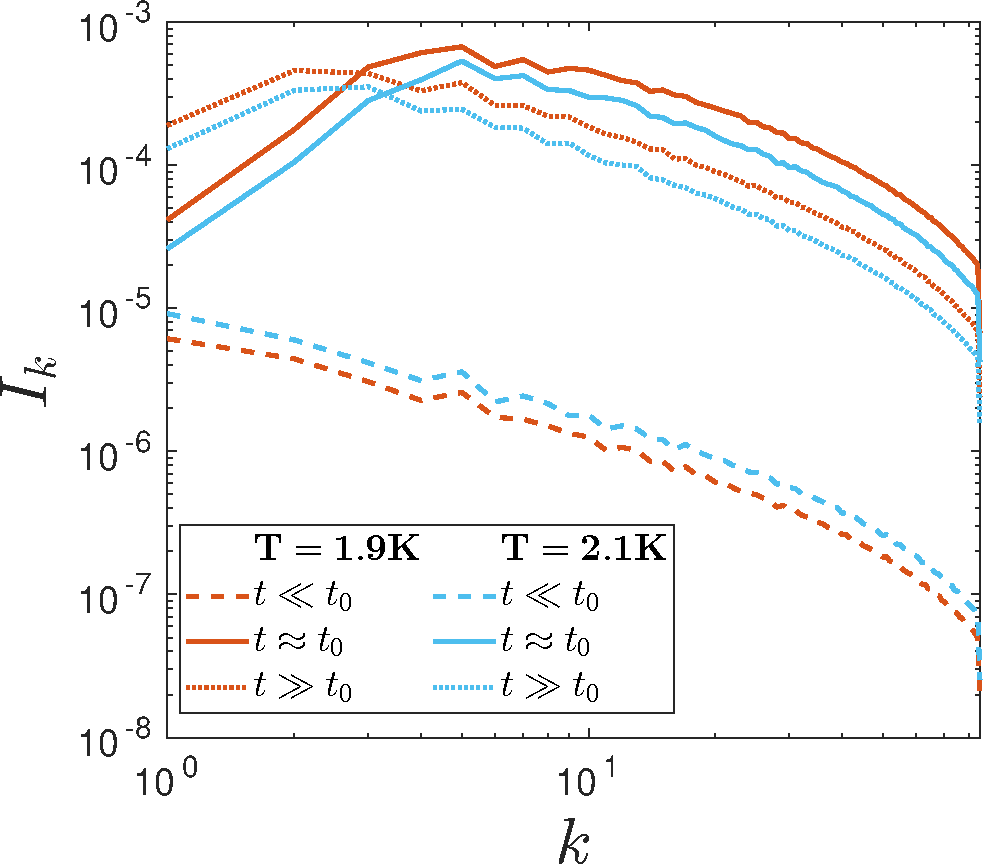
\includegraphics[width=0.4\textwidth]{inj-spec.pdf}
    \end{figure}

    To clarify this point, we have included a supplementary figure showing the injection spectrum, which demonstrates how it complements the energy flux and spectrum, thereby resolving the apparent discrepancy. We have also updated Fig.3a to ensure consistency with the scaling used throughout the manuscript. \\   
    %We will also include a brief explanatory note in the revised manuscript to ensure this is clear to readers.


    \refcomment{4) p.4, right, "This inverse energy transfer arises from the helical
    character of the friction generated by the Kelvin waves released by
    the reconnecting cusp": Is the inverse energy transfer due to the
    Kelvin wave? This reviewer thought that it is due to the mutual
    friction force being helical as described on the left of p.4.}
  
    \refcomment{5) Figure caption in Fig.1, $(t - t_0)/\tau_R$: $t_0$ is $t_R$ ?}

    The value $t_0$ should in fact be $t_R$, the typo has been corrected.\\
    
    \refcomment{6) Horizontal label in Fig.2: $(t - t_R)/\tau_R$ would be better than $(t- \tau_R)E_R^{1/2}/L_R$ ?}

    The authors agree with the comment of the referee that the current notation is not ideal. Instead, the figures have been changed to use the timescale in the horizontal axis of all time plots. Additionally to note, we have replaced the vertical axis label of Fig. 3b with $E_R/\tau_R$, simply a change of symbols to make clear the non-dimensionalisation of units.\\
    
    \refcomment{7) Figure 3(a): Is there a power law for the slope of $E(k)$?}

    The figure has been updated with a power law of $k^{-3}$.\\
    
    \refcomment{8) p.4, left, "From Fig. 4 we determine the non-dimensional
    timescale...": Please describe the meaning of $t^*$.}

    The time $t^*$ was introduced as the time at which we observe a sufficient decay of the helical force ratio, where the difference is around 5\% between the positive and negative modes and remains relatively stable afterwards. In order to make this clearer, we have added a sentence in the text to explicity state this.

    \refcomment{9) p.4, left, "corresponding dimensionally to $\tau = 0.1$s for both
    temperatures.": Please describe where "$\tau = 0.1$s" comes from or what
    that means. Is the time when the helicity is changing?}
    
    The value of 0.1s comes from dimensionalising the values of $\tau=0.01$ for $T=1.9K$ and $\tau=0.005$ for $T=2.1K$, using the values of $\tilde{\tau}$ listed in the supplementary materials. \\
    
    \refcomment{10) Reference 53: B. ME should be M. E. Brachet. The year of 2026
    should be 2017.}

    Incorrect reference corrected as noted by the reviewer.\\

\subsection*{Referee B}

\refcomment{The authors’ main motivation, as far as I understand, is to propose a mechanism for the inverse energy cascade which is numerically observed in counterflow superfluid turbulence [Polanco and Krstulovic, PRL (2020)].}

We want to clarify to the Referee that the purpose of our work is not at all to explain Polanco \& Krstulovic PRL 2020. Indeed, this article is only cited at the end of our manuscript, as a possible physical setting where the new physical phenomena described in our manuscript could be relevant, and it could be perhaps at the origin of the inverse cascade reported in that paper (that one of us co-authors).  To avoid possible confusion, we have reformulated the only paragraph in the conclusion where we cite Polanco\&Krstulovic.\\

\refcomment{As recalled by the authors, inverse energy cascades show up when helicity symmetry is explicitely broken by external forcing as in [Plunian et al., JFM (2020)]. Their claim, then, is that vortex reconnection events in superfluid turbulence will similarly break helicity symmetry and trigger, in this way, an inverse energy cascade in the flow.}

Regarding this point, the referee understood the most important claim of our paper concerning the sign-defined helicity injections. We would like to highlight that we have consciously avoided talking about the inverse energy cascade, as we are well aware that our system is not turbulent. We have used the words “inverse energy transfers” instead.\\

\refcomment{While the paper’s idea is interesting and worth pursuing, I believe the authors fail to provide even minimal evidence to support their case. Below, I address my main points.
(i) First, the use of the word “turbulence” in the very first line (and used 16 times in other parts) of the manuscript is misleading: the flow studied by the authors is just a collision of vortex filaments. There is no turbulent flow at all here. It is all about a specific problem on superfluid flow instability.}

As the Referee is certainly aware, vortex reconnections play an important role in turbulence.  We have never claimed that our system is turbulent, but we do think that our findings have a strong impact on quantum turbulence.  As the Referee might have noticed while counting how many times we used the word “turbulence”, we only used it in the introduction to motivate our work and to explain its relevance to a broad audience, and at the very end of our manuscript end to comment on its implications in the conclusions. Explaining cascades and then turbulence is necessary to understand the role of helicity on transfer towards large scales. We still believe that the use of the word turbulence is appropriate in our manuscript. We have nevertheless added a sentence in the introduction to remind the reader of the importance of vortex reconnections in turbulent flows and a comment in the conclusions about when our finding might be important for quantum turbulence. \\

\refcomment{(ii) The work of Polanco and Krstulovic [PRL (2020)] gives strong indication that counterflow superfluid turbulence behaves (for large enough counterflow velocities) as a quasi two-dimensional syste and, therefore, an inverse energy cascade is expected to occur. Polanco and Krstulovic have also observed, by the way, the energy spectrum decay of the direct enstrophy cascade, in further qualitative agreement with the Batchelor-Kraichnan picture of 2D turbulence.}

We do agree with the Referee’s understanding of Polanco\& Krstulovic main result. However, we do not understand why the Referee mentions it as they have not formulated any question or critcism.\\

\red{\textbf{GK: Something better to say?}}

\refcomment{(iii) The helicity production for an individual vortex reconnection event can be, of course, positive or negative. However, it is unlikley that this will be the case for the global helicity production associated to the complex vortex tangle of counterflow turbulence. I note that the previous results of [Plunian et al., JFM (2020)] refer to flow regimes where helicity symmetry is broken across all scales by the external forcing.}

Indeed, the helicity injection produced by random vortex reconnections is not sign-defined, but by a single one, it is.  In isotropic turbulence, the helicity injection produced by vortex reconnection is certainly positive and negative. In the case when the system is highly anisotropic and the vortex density is sufficiently large, it is less clear if such a symmetry breaking could favour the production of helicity of one given sign. For this reason,  at the end of the conclusion, we mentioned counterflow turbulence as such an example and raised the question of whether the findings of Polanco\&Krstulovic could be ultimately related to the new mechanism reported in our Letter.  Providing a definitive answer to this open question is undoubtedly challenging and beyond the scope of our work. In the revised version, we have softened and reformulated the sentence referring to Polanco\&Krstulovic.\\

\refcomment{(iv) The vortex reconnection mechanism for the inverse energy cascade would imply that energy would flow from very small scales (around the atomic sizes of the vortex cores) towards the integral length scales. That is not what is observed, as discussed by Polanco and Krstulovic [PRL (2020)].}

We remind the Referee that Polanco\&Krstulovic used the HVBK model. This model does not describe quantised vortices, and the energy injection was made through an external term, which acting scale can be chosen arbitrarily.  The inverse cascade is triggered by the nonlinear term when the counterflow is strong enough, which leads to a strong anisotropy. In our coupled model, the normal fluid energy injection is produced by vortex reconnections, and it is indeed transferred towards large scales.  We remind the Referee that one needs to be careful while comparing HVBK and our couple model as they describe the physics at very different scales.  Again, by writing the sentence about Polanco\&Krstulovic, we simply raise a question that needs further investigation.\\

\refcomment{(v) Finally, the “inverse energy cascade” detected by the authors may be unrelated to helicity production. One could just as easily argue that the perturbation/production of the standard component of the fluid through vortex reconnection is initially local- ized around the point where the filaments come into close contact. Subsequently, this normal component perturbation is strained by the specific background velocity configu- ration of the surrounding normal fluid. Helicity would not play any relevant dynamical role here.}

The Referee has raised a good point.  In a recent paper [arXiv:2501.08309 ], three of us studied the wakes generated by moving superfluid vortices (with respect to the normal fluid). In this case, energy is transferred to small scales, discarding the scenario proposed by the Referee.\\

\red{\textbf{GK: Shall we add a comment like this in the letter? GK:a figure in the suplemental? }}\\

\refcomment{For the above reasons, I do not recommend the paper for publication in the PRL.}

We hope that we have provided enough arguments to the Referee and they see now the impact of our Letter.







\end{document}
